As explained in section \ref{intro:newway} of the introduction chapter, one aspect that deserves special attention when teaching Japanese is the \textbf{importance} of a word or Kanji. Importance can be defined in a number of ways, such as the definition implied by the grade lists brought forward by the Japanese Ministry of Education, the Ky\={o}iku Kanji, which were introduced at section \ref{intro:presentapproaches}. This grading system uses a constructivist approach, where Kanji that hold more simple and concrete meaning are taught earlier than Kanji that represent more complex or abstract ideas. Additionally, the Ky\={o}iku Kanji grades also reflect the frequency which characters are expected to be present in text compatible with the age of the student in question\footnote{For example, a student learning first grade Kanji should be around six years old, and therefore be presented more often with text where the concepts, and therefore the Kanji, are simple}.
Although this specific order proves itself useful when teaching native Japanese children, it is not necessarily the best order to teach foreign adults that are seeking to learn Japanese as an additional language.

Taking these cases in mind, we propose that for adults, a much more concerning factor in deciding which Kanji should be tackled first and with more seriousness\footnote{In here, we assume that the study technique will be similar to a factorial method: the student will learn one topic and progress to learn other topics returning from time to time to check if the first concepts are clear. If this is the method used in a web app to teach Japanese, the first Kanji to be taught would also coincide with those that are expected to be the best understood} would be the relative frequency this Kanji is used in media that he is likely to be interested in. It is important to note that the order proposed in this chapter is not the final order that would be advised to be used in the study of Japanese Kanji, but only a stepping stone in the direction of obtaining this better list. Chapter \ref{chap:graphs} elaborates more on other factors that should be considered when estimating the importance of a Kanji character.

In the next sections, we describe the process of seeking an appropriate source of data, we compare the total word distribution and Kanji-only distribution to a power log distribution (also known as Zipf's distribution) and finally we explore the implications of the relationship of the specific format of the frequency distribution curves and the learning process of a student.

\section{Frequency estimation of Japanese text}
Japanese has a number of particularities that make the frequency estimation of words (or lemmas) to be unique, and should be explained in order to understand the complexity and steps of the process.

\subsection{Parsing the Japanese Language}\label{freq:parsing}
The Japanese language does not use the concept of blank spaces in its writing system, although it does use some punctuation marks such as commas, periods and exclamation marks. That being so, the task of reading Japanese also comprises the task of determining the start and end of words and syntax particles.
As an example, let us examine a simple sentence in Japanese: The cat is sitting on the roof.

\begin{center}
\jap{猫が屋根に座っている}
\end{center}

Firstly, it can be noted that there are ten graphemes in this sentence, but no spacing marks, as mentioned earlier. Now, let us artificially introduce space marks along with a r\={o}maji transliteration\footnote{refer to Section \ref{ape:romanization} in the Appendix for more information about the romanization process} below.

\begin{center}
\jap{猫 が 屋根 に 座っている}\\
neko ga yane ni suwatteiru
\end{center}

With this, we identify five separate words in this sentence. It was possible to do the parsing of this sentence due to the previous knowledge of the structure of Japanese sentences and the function each word plays in the sentence. Initially we read the Kanji \jap{猫}, which is read as neko and means "cat", we identify this as an individual word of the sentence and expect the next element to be a syntax particle, designing the function of this element in the sentence. In succession, we find the Hiragana \jap{が}, ga, the subject marker, which indicates that "cat" is the subject. We then proceed to look for the predicate of this sentence and find the word with two Kanji \jap{屋根}, yane, which means "roof". We then expect to see a direct or indirect object particle marker, and thus we find the Hiragana \jap{に}, ni, the indirect object marker. Finally we expect to find the verb of the sentence
\footnote{Japanese is structured around Subject/Object/Verb, instead of the form Subject/Verb/Object, which is more common in western languages}, 
and read the Kanji accompanied by some Hiragana stem \jap{座っている}, suwatteiru, the verb "to sit" in the present progressive form.

This task of identifying word boundaries is much facilitated by the intermixing of Kanji, Hiragana and occasionally Katakana in sentences, which is one of the reasons that makes Kanji so useful for the Japanese language.

\subsection{Lemma extraction (optional)}

Optionally, the occurrence of elements can be done around lemmas instead of words. Lemmas are the unification of multiple words under a same root such as the uninflected forms of words. With this process, different representations of the same concept can be condensed to a unique entry, instead of having it spread in multiple entries. In English the process would be similar to unifying the words \textit{"moves"}, \textit{"moving"} and \textit{"moved"} to the word \textit{"move"}. Figure \ref{fig:lemmas} exemplifies the process in English and Japanese. In the case of the Japanese language there's an additional issue that may be solved, which is the unification of homographs under a same lemma. For example, both spellings \jap{お勧め} and \jap{お薦め} are valid ways to write \jap{おすすめ}, osusume, which means recommendation.

\begin{figure}[ht]
    \begin{subfigure}{0.5\textwidth}
    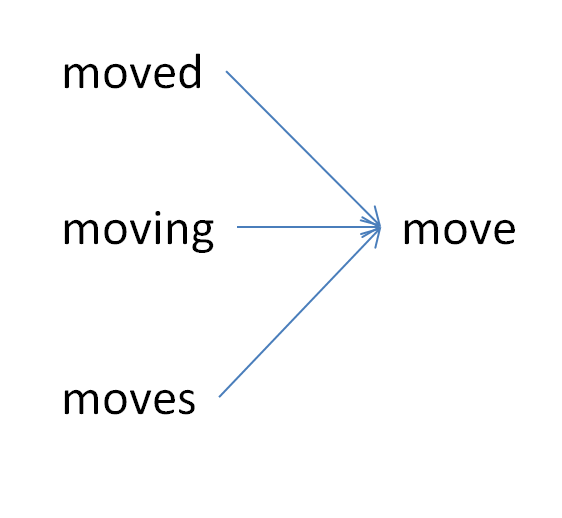
\includegraphics[width=0.9\linewidth]{Cap2/LemmaEnglish}
    \caption{Lemma extraction in English.}
    \label{fig:lemmaeng}
    \end{subfigure}
    \begin{subfigure}{0.5\textwidth}
    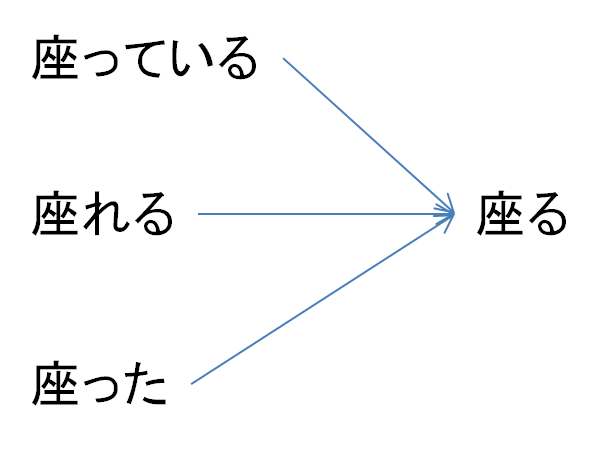
\includegraphics[width=0.9\linewidth]{Cap2/LemmaJapanese}
    \caption{Lemma extraction in Japanese.}
    \label{fig:lemmajap}
    \end{subfigure}
    \caption{Comparison of lemma extraction in English and Japanese.}
    \label{fig:lemmas}
\end{figure}

\section{Projects that estimate word frequencies}
A variety of different projects undertake the mission of determining which are the most common words in the Japanese Language. Each of the next three presented projects were taken from a different type of media.

\subsection{Alexandre Girardi's analysis of newspaper data}
This is the oldest of the three projects, dating to 1998, and was taken from parsing 4 years of the newspaper Mainichi Shinbun (\jap{毎日新聞}, literally "Daily Newspaper"), in a total of 74,721,217 occurrences spread among 311,049 words\cite{monash}. This is the most widely used project when estimating Kanji frequency rank, since this rank is already in built in a number of open source projects, including the most widely used open-source dictionary of Japanese words, Jim Breen's WWWJDIC\cite{breen2000japanese}. Alexandre Girardi's project has four main problems: first, the fact that the type of speech used in newspapers in Japanese is radically dissociated from the common day-to-day written form of Japanese. A second issue is that it is skewed to some few topics, such as economy, politics and weather forecast. The third issue is that this project is based around word extraction, instead of lemma extraction. Finally, a fourth issue is that the methodology used in this project was not clearly published by Alexandre Girardi, limiting itself to some few lines in a readme file.

\subsection{Wikitionary analysis of a Japanese Wikipedia dump}
The project in question was drawn from a complete dump of the Japanese Wikipedia on April 22th, 2015, using the morphological analyzer MeCab\cite{kudo2005mecab} and cleaning the end results to unify words under lemmas, yielding a total of 669,419,716 occurrences spread among 2,610,776 lemmas\cite{wikitionary2015wordfreq}. It is important to note that a great number of lemmas appears only one or two times. A great number of this rare lemmas are attributable to Hiragana transliterations of Kanji words inside parenthesis, a phenomena that is customary for the first sentence of each article. For example, the article about the Japanese language starts with:

\begin{center}
\jap{日本語(にほんご、にっぽんご)は、}
\end{center}

As we can see, this article starts by writing "Japanese Language" in Kanji, followed by two different possible readings for this word. In this case, since a sequence of Hiragana can be usually converted to a number of different words with different meanings, the lemma extraction failed to unify these with the lemmas containing Kanji.

If we limit the examples only to lemmas that appear more than once, the total number of occurrences is reduced to 668,024,047 occurrences over 1,214,107 lemmas. If we limit to only lemmas with at least three samples, the total number of occurrences is then reduced to 667,301,019 occurrences over 853,593 lemmas. As it can be noted, each step in this direction reduces the total number of occurrences by only a small fraction, while the number of words drops quickly in comparison with its scale. This project can be seen as as improvement over Alexandre Girardi's project for its sheer size (over 669 million \textbf{lemmas} occurrences on this project, while the previous one was resumed to only 74 million \textbf{words} occurrences) and the fact that it does lemma unification. However, the written form usually used in Wikipedia is also of a different sort than the form of speech that would be more expected to see in day-to-day texts for its formality, and it also presents a imbalance of terms, this time toward date related Kanji (the Kanji for year is specially oversampled), as well as descriptive terms. Also, simple concepts such as the Kanji for "ear" and other very simple Kanji are specially undersampled, since they represent simple concepts that are not useful in explaining other concepts.

\subsection{Christopher Brochtrup's analysis of Japanese novels}
In 2007, Christopher Brochtrup created a tool called the "Japanese Text Analysis Tool"\cite{christopher2007tool}, for the analysis of arbitrary Japanese texts, including an inbuilt capability of doing morphological parsing of texts through the MeCab\cite{kudo2005mecab} analyser followed by a word frequency report, along with other functionalities. To present as an example of this tool, on May 27th, 2012, he created a report from 5000+ Japanese novels that were in public domain\cite{christopher2007wordfreq}. This analysis was done by lemma reduction to root forms of conjugated words, but with no attempt to unify different spellings of words under one type of writing. This analysis counted a total of 366,120,879 occurrences, spread over 193,121 lemmas. It is a matter of course that this project also shows an imbalance toward words more commonly used in novels, but a comparative analysis of Kanji rank versus Japanese grade did not show any significant problems. As for its size, it is composed of almost 5 times the number of occurrences in the newspaper data and about half the number of occurrences of the Wikipedia project. These are spread over only 193 thousand lemmas, a number much more closely related to the expected size of a language vocabulary.

\subsection{Final choice and considerations}
Each of the presented projects have its own implementation and data-cleaning process particularities, but all of them fall victim to the same shortcoming: being single-sourced.

The relative frequency of words holds a strong dependence with the media at which it is published in. That being the case, the most appropriate choice would be taking multiple sources and conjoining them in a manner as to respect their individual scale of total words and to keep the statistical properties of each project, also adjusting each to be centered around the same lemma creating strategy, instead of a word-listing fashion. An even greater enhancement would be aggregating even more sources of data, and classifying those in respect of topics, interests and expected readers age group, so that a different frequency distribution could be generated for each class of user profile, specifically tailored to that profile's tastes and needs.

Since this task of pluralizing the sources of data was considered to be outside the scope of this academic work, it was not executed and is proposed as a possible improvement over the results presented in this work. Instead, we choose the media that was the most expected to be useful to an adult learner with broad interests: \textbf{we choose to use Christopher Brochtrup's analysis of Japanese novels}. That being the case, we will be optimizing the learning experience of a student that tries to read Japanese novels. It is important to note that since this decision was in some sense arbitrary and therefore may be expected to change in a future step of this project, the back-end of the analysis framework developed was designed in a way that does not make any assumptions about the origin of the lemma-count pairs, so that this source could be easily replaced with any other project that provides words in the format "count,word(or lemma)" in a .csv file.

\section{Zipf's Law}
The Zipf law is an empirical law that states that given the evolution of a natural language, the frequency of any given word is approximately proportional to its rank in a biggest-to-lowest frequency table, a rule also known as the power law. It is generally recognized as so since it was popularized by the American linguist George Kingsley Zipf\cite{zipf1935psycho}. His work comprised a hand counting and later on a log-log analysis of James Joyce's book Ulysses. Zipf noticed that in this graph the series of points seemed to from an apparent downward straight line, giving rise to the law enunciated above, or in a more technical fashion in equation \ref{eq:zipf}.

\begin{equation}\label{eq:zipf}
    f(r)\propto1/r^\alpha
\end{equation}

Where \(\alpha \approx 1\). A generalization of this law that more closely fits the frequency distribution in languages was proposed by Mandelbrot\cite{mandelbrot1962paretian}, and is expressed in equation \ref{eq:mandel}.

\begin{equation}\label{eq:mandel}
    f(r)\propto1/(r+\beta)^\alpha
\end{equation}

Where \(\alpha \approx 1\) and \(\beta \approx 2.7\). While the original equation portrays a perfectly straight line in the log-log graph, the Zipf-Mandelbrot equation yields a downward facing curve formed by the connection of two approximately straight lines. The behaviour of this \(\beta\) parameter is exemplified in figure \ref{fig:mandelbrotbeta}.

\begin{figure}[ht]
    \centering
    \begin{subfigure}{0.475\textwidth}
    \centering
    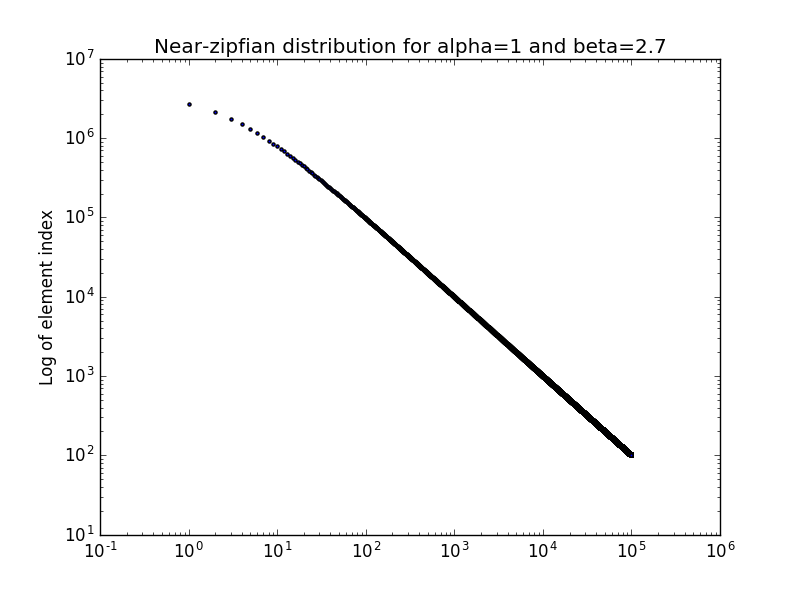
\includegraphics[width=0.9\linewidth]{Cap2/zipf27}
    \caption{Using \(\beta = 2.7\).}
    \label{fig:zipf27}
    \end{subfigure}
    \begin{subfigure}{0.475\textwidth}
    \centering
    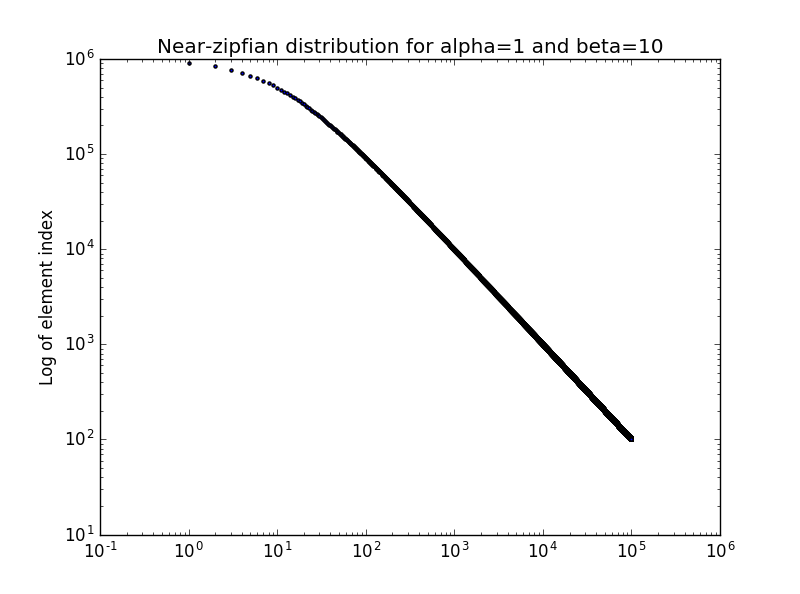
\includegraphics[width=0.9\linewidth]{Cap2/zipf10}
    \caption{Using \(\beta = 10\).}
    \label{fig:zipf10}
    \end{subfigure}
    
    \begin{subfigure}{0.475\textwidth}
    \centering
    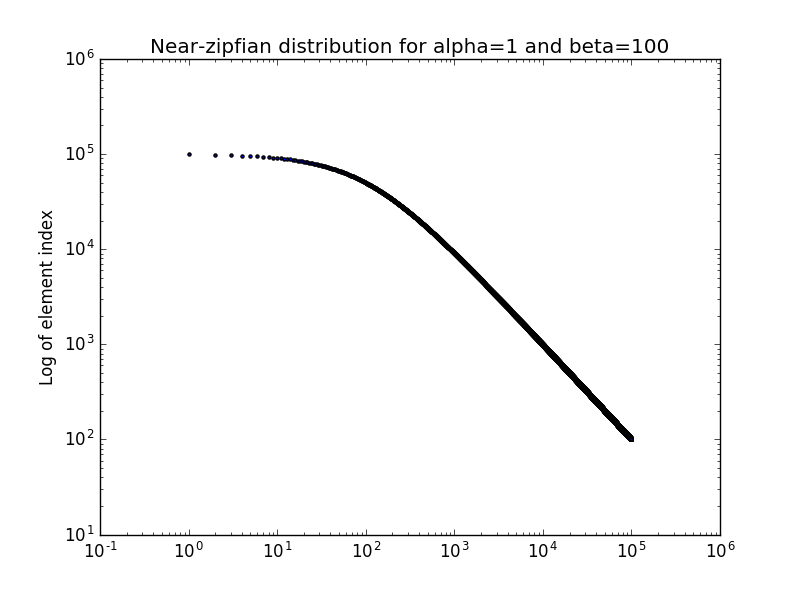
\includegraphics[width=0.9\linewidth]{Cap2/zipf100}
    \caption{Using \(\beta = 100\).}
    \label{fig:zipf100}
    \end{subfigure}
    \begin{subfigure}{0.475\textwidth}
    \centering
    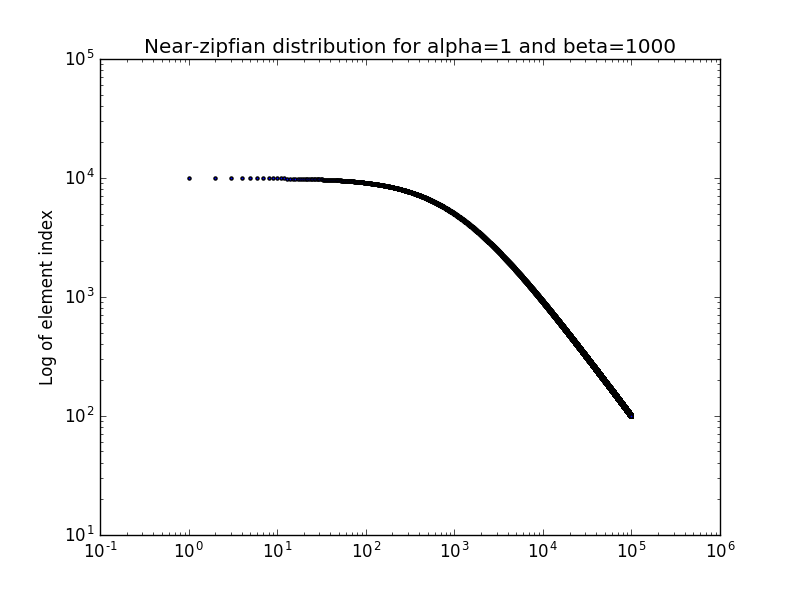
\includegraphics[width=0.9\linewidth]{Cap2/zipf1000}
    \caption{Using \(\beta = 1000\).}
    \label{fig:zipf1000}
    \end{subfigure}
    
    \caption{Log-Log graphs of data produced according to Zipf-Mandelbrot equation with various parameters.}
    \label{fig:mandelbrotbeta}
\end{figure}

As it can be seen in this sequence of four figures, as the parameter beta increases the fall of the curve is delayed.

Although a number of possible explanations were given about the origin of this phenomena, with a number of different deductions from base principles arriving at this same formula, very few of these theories focus themselves in giving testable accounts of which should be the right theory for the psychological mechanisms responsible for this effect\cite{piantadosi2014zipf}. 

In the subsequent sections we will analyse a number of frequency distribution and will do various analysis of the shape of the Log-Log graphs of these distributions. Although a more rigorous scrutiny over the presence of absence of power log behaviour would be possible through mathematical tools\cite{newman2005power}, we will focus on a simple visual analysis of the curve, giving more emphasis to the basic insights that these can bring.

\section{General Word Distribution}\label{freq:word}

Using Christopher Brochtrup report, the process of creating a \(occurrence \times rank\) graph is very straight forward. We simply produce the scatter plot of the occurrence of lemmas versus their rank in a sorted list where their counts are decreasing with the increase of their rank. The result of this analysis on linear and log-log scale is presented on Figure \ref{fig:lemmacount}.

\begin{figure}[ht]
    \centering
    \begin{subfigure}{0.475\textwidth}
    \centering
    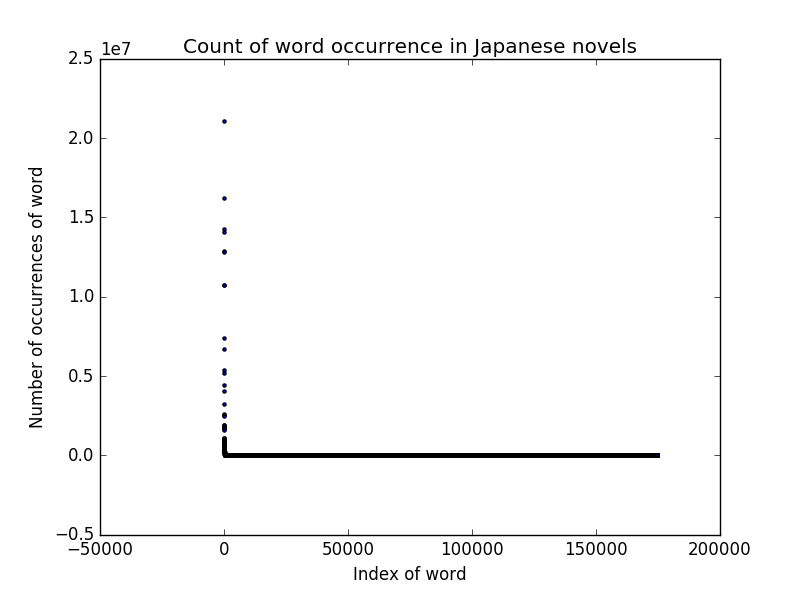
\includegraphics[width=0.9\linewidth]{Cap2/WordCountNovels}
    \caption{Linear distribution of lemmas.}
    \label{fig:lemmalinear}
    \end{subfigure}
    \begin{subfigure}{0.475\textwidth}
    \centering
    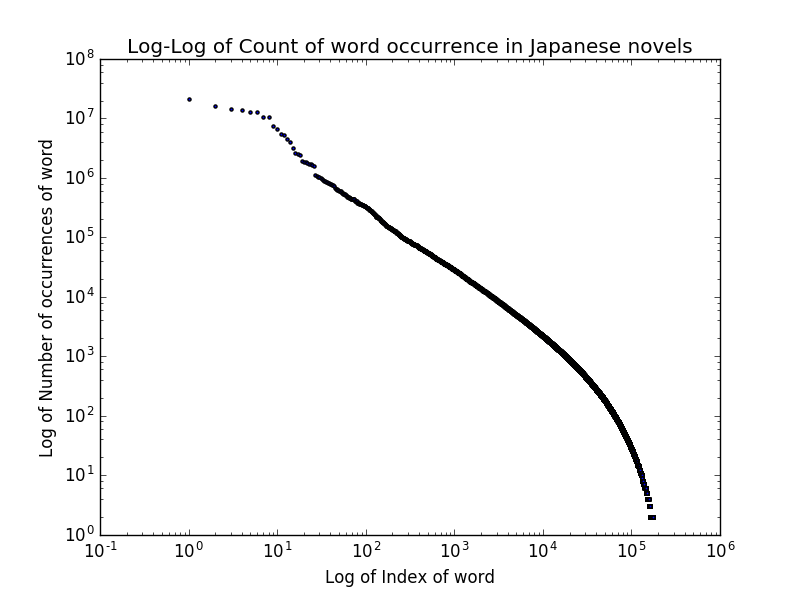
\includegraphics[width=0.9\linewidth]{Cap2/LogLogWordCountNovels}
    \caption{Log-Log of the distribution of lemmas.}
    \label{fig:lemmalog}
    \end{subfigure}
    
    \caption{Distribution of lemmas used in Japanese Novels.}
    \label{fig:lemmacount}
\end{figure}

The linear graph does not bring much insight except for the expected fact that the first few words appear a lot, with a long tail of lemmas that only happen a few times. Upon inspection of the Log-Log graph, we are able to more concretely grasp the exchange rate between the rise of the index and the fall of the number of occurrences of words takes place. In this case, we can visually detect that the curve has a Near-Zipfian behaviour, with most of the core part of the curve closely matching a straight curve. This was to be expected, since most human languages were already observed to be closely related to power log curves.

\section{Distribution of Words with Kanji}\label{freq:wordwithkanji}

We can now refine our earlier data-set so that it is exclusively formed by words with at least one J\={o}y\={o} Kanji, keeping the ordering as was done in the previous section. The result of this analysis is presented in Figure \ref{fig:lemmacountwkanji}.

\begin{figure}[ht]
    \centering
    \begin{subfigure}{0.475\textwidth}
    \centering
    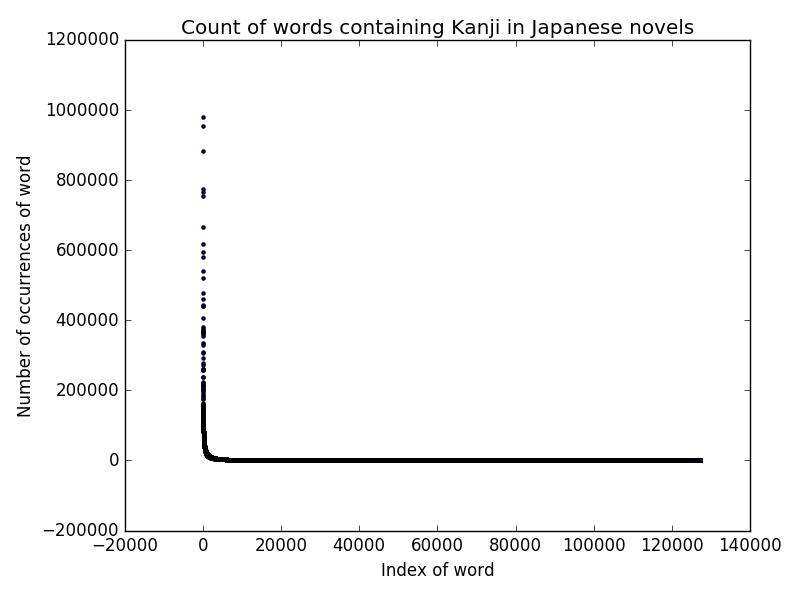
\includegraphics[width=0.9\linewidth]{Cap2/WordCountWithKanjiNovels}
    \caption{Linear distribution of lemmas.}
    \label{fig:lemmalinearwkanji}
    \end{subfigure}
    \begin{subfigure}{0.475\textwidth}
    \centering
    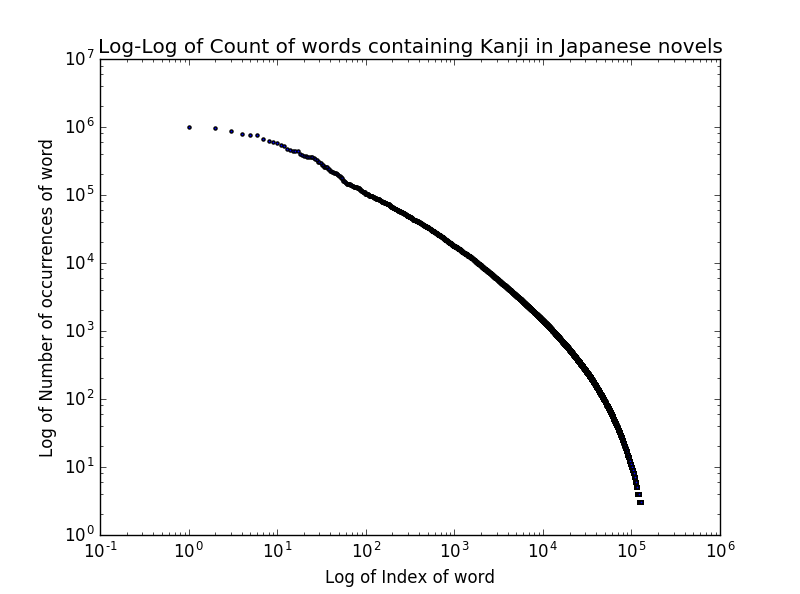
\includegraphics[width=0.9\linewidth]{Cap2/LogLogWordCountWithKanjiNovels}
    \caption{Log-Log of the distribution of lemmas.}
    \label{fig:lemmalogwkanji}
    \end{subfigure}
    
    \caption{Distribution of lemmas used in Japanese Novels that contain at least on Jouyou Kanji character.}
    \label{fig:lemmacountwkanji}
\end{figure}

Once again, we note that the linear plot is only able to bring the expected insight that the occurrences of lemmas are highly concentrated in the fist few. Now, upon scrutiny of the Log-Log graph, we observe a slight curving of the plot in the direction of the upper right corner, indicating a slightly different behaviour for this subset. This outward moving of the center of the curve indicates that words containing Kanji tend to be more frequently used than it would be expected of them if they represented the totality of components from a language that follows a power log curve with great fidelity.

\section{Jouyou Kanji Distribution}\label{freq:kanji}

Finally, we can take the subset of words in the last chapter and proceed to invert the center of counting to be around Kanji, instead of being around lemmas. Since we already start the process knowing which are the 2,136 Kanji that should be counted, the task resumes itself on creating a python Counter object (a hash map of string to int) and adding the number of times its host word occurs. This task was performed while simultaneously gathering example words for each Kanji, but for simplicity we present a fictitious code that would perform only the task of inverting this count.

\begin{minted}{python}
import collections
import IS  # Important structures defined for this project.
import IP  # A collection of relevant paths for this project.
import toolbox  # A toolbox to perform useful tasks.

def create_kanji_counter():
    # count_words is a tuple (count, word)
    count_words = toolbox.load_data(IP.WORDS_FILTERED)
    kanji_counter = collections.Counter()
    for c_w in count_words:
        for character in c_w[1]:
            # Checks if the word is in an alternative form
            if character in IS.equiv_to_jouyou:
                character = IS.equiv_to_jouyou[character]
            # a set containing the Jouyou Kanji
            if character in IS.jk_set
                kanji_counter[character] += int(c_w[0])
    return kanji_counter
\end{minted}

Using the generated \textit{kanji\_counter} object we can now analyse the relationship between the frequency of a Kanji and the total number of times it occurred. These graphs are presented in Figure \ref{fig:kanjicount}.

\begin{figure}[ht]
    \centering
    \begin{subfigure}{0.475\textwidth}
    \centering
    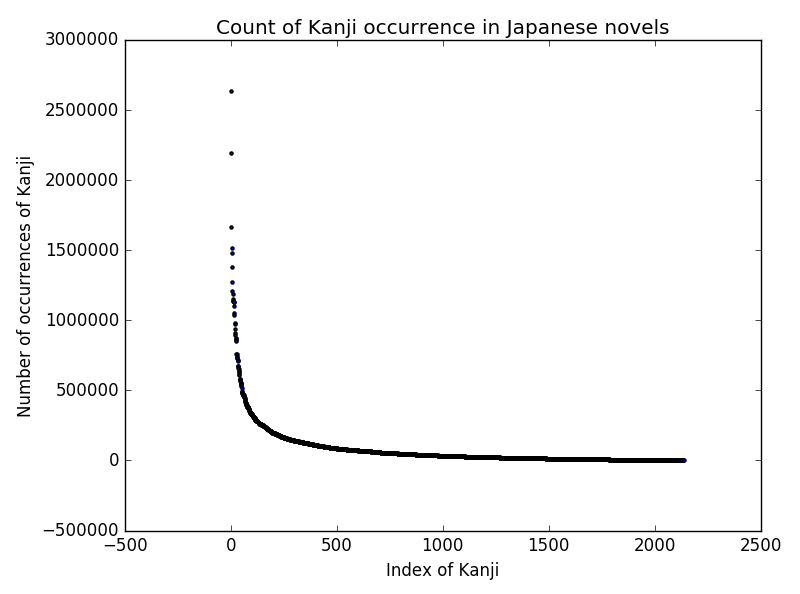
\includegraphics[width=0.9\linewidth]{Cap2/KanjiCountNovels}
    \caption{Linear distribution of Kanji.}
    \label{fig:linearkanjicount}
    \end{subfigure}
    \begin{subfigure}{0.475\textwidth}
    \centering
    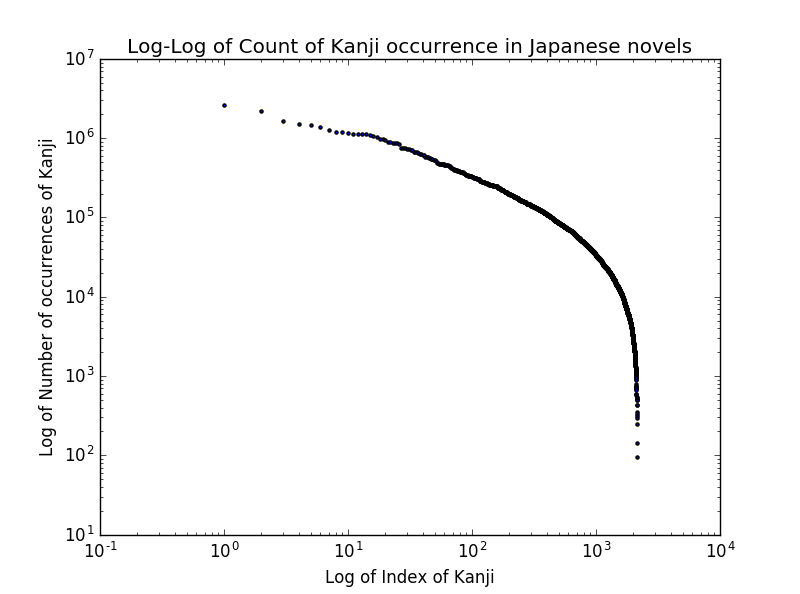
\includegraphics[width=0.9\linewidth]{Cap2/LogLogKanjiCountNovels}
    \caption{Log-Log of the distribution of Kanji.}
    \label{fig:logkanjicount}
    \end{subfigure}
    
    \caption{Distribution of Jouyou Kanji usage in Japanese Novels.}
    \label{fig:kanjicount}
\end{figure}

Once more, the linear graph is just auxiliary to the conclusion that a few of the elements concentrate most of the occurrences, but now we observe a smoother transition from the initial number of examples to the tail of the curve. This behaviour can be even more easily noticed in the Log-Log graph, where a curve that distances radically from a power log curve was created. In the specific case of Kanji, we note that the number of occurrences supports itself high even with an increase of rank from the Kanji approximately until the \(10^3\) mark. After this point, the distribution abruptly falls in number of occurrences for small logarithmic increments in the index.

This characteristic could be explained by the fact that the list of Jouyou Kanji was artificially created by the Ministry of Education in Japan, instead of forming over the pure necessity of users, as is the evolution process of a language and as it is still observer for general Japanese words. The Kanji chosen by the Japanese Government followed basically two rules, which could explain the two different sections of the occurrence graph:

\begin{enumerate}
    \item Kanji that represented frequently used concepts.
    \item Kanji that were already in use in legal documents from the government. This need arose from the strict rule that all public documents should be written exclusively with Jouyou Kanji. To accommodate this rule, Kanji that were obscure but were used in the legal jargon were introduced in the Jouyou Kanji list.
\end{enumerate}

To better elucidate this concentration of uses in a few Kanji, we generated an alternative view for this case. By dividing the number of occurrences by the total number of Kanji surveyed, we were able estimate the frequency of each Kanji as a fraction between 0 and 1. Furthermore, by adding each element with its previous frequency, we generated a cumulative distribution function of the use of Kanji. This CDF is presented in Figure \ref{fig:cdfkanji}.

\begin{figure}[hb]
    \centering
    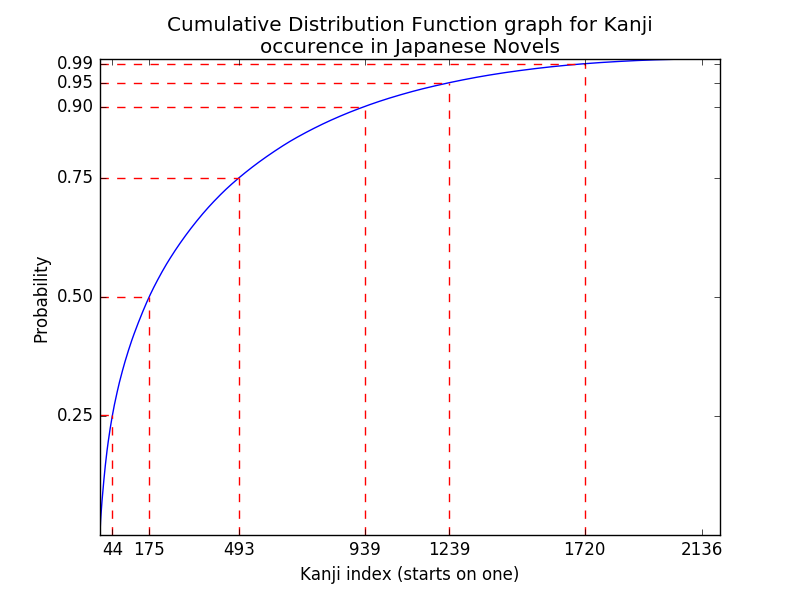
\includegraphics[width=0.8\linewidth]{Cap2/CDFKanji}
    \caption{Cumulative Distribution Function for the use of Jouyou Kanji in Japanese Novels}
    \label{fig:cdfkanji}
\end{figure}

The red references show the number of Kanji to be learned to reach some certain statistical level. As an example, it can be noted that 175 of the 2,136 Jouyou Kanji account for 50\% of the total occurrences of Jouyou Kanji in the surveyed novels. A deeper interpretation of this numbers will be presented on Section \ref{freqs:interpretation}.

\section{Comparing study efforts on pure frequency versus Kyouiku Kanji order}

As a base of reference, we will now proceed to study the distribution of the grades assigned by the Japanese Government for the Kyouiku Kanji list. Since no order is defined inside each of these six grades, we proceed to analyse the study of a student under the best-case scenario\footnote{although the student limits itself to proceed studying Kanji one grade at a time, he does so studying the most common Kanji first.} and the worst-case scenario\footnote{In this case, the student limits itself on the grades and study the least frequent Kanji first}. A representation of this curve on the best-case and worst-case scenarios is depicted in Figure \ref{fig:cdfgrade}.

\begin{figure}[ht]
    \centering
    \begin{subfigure}{0.9\textwidth}
    \centering
    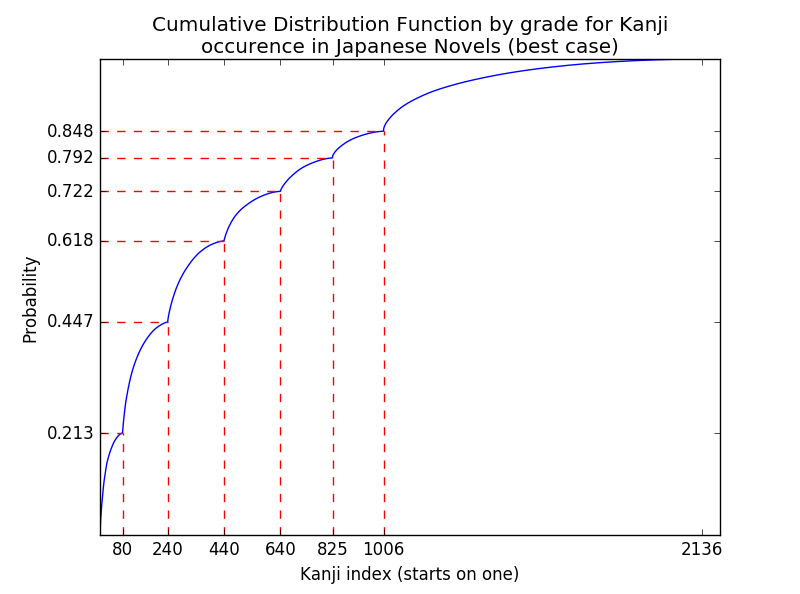
\includegraphics[width=\linewidth]{Cap2/CDFGrade}
    \caption{Best case scenario.}
    \label{fig:cdfgradebest}
    \end{subfigure}
    \begin{subfigure}{0.9\textwidth}
    \centering
    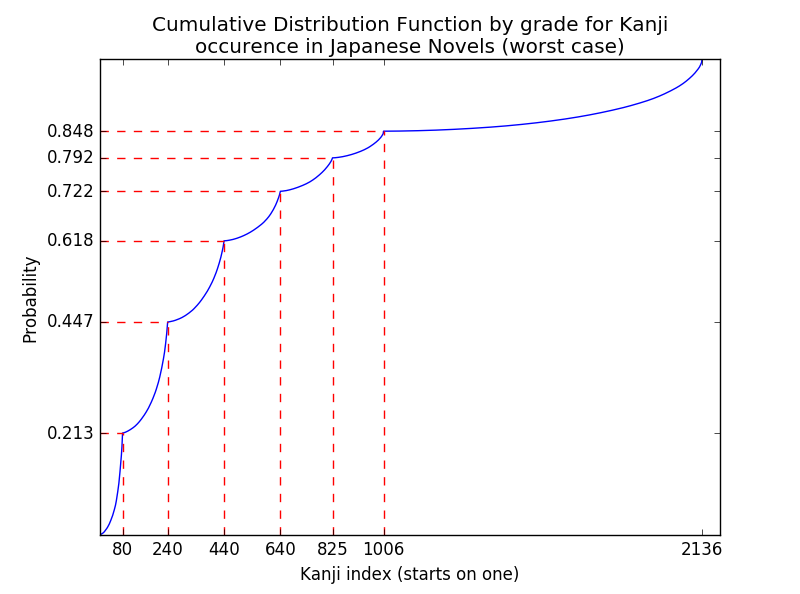
\includegraphics[width=\linewidth]{Cap2/CDFGradeWorst}
    \caption{Worst case scenario.}
    \label{fig:cdfgradebestworst}
    \end{subfigure}
    
    \caption{Cumulative Distribution Function limited by the grades determined in the Kyouiku Kanji.}
    \label{fig:cdfgrade}
\end{figure}

The reference lines in this case represent the number of Kanji to be studied in each grade and the corresponding expected value for the cumulative frequency up to that point. An example of this interpretation would be to state that after learning all the 1006 Kanji from primary school, a Japanese student is expected to recognize 84.8\% of the Kanji characters in a Japanese novel. As it could be expected, between the best and worst case scenarios the inflection points remain stable, representing the cumulative probability gain for each grade. The curves differ in each other inside grades and after the end of primary school in its concavity.

To better compare the study of a native Japanese following the grade lists and a student that uses the order implied by the relative frequencies of Kanji characters, those two curves were plotted together in Figure \ref{fig:cdfcomparison}, again separating in best and worst case scenarios.

\begin{figure}[ht]
    \centering
    \begin{subfigure}{0.9\textwidth}
    \centering
    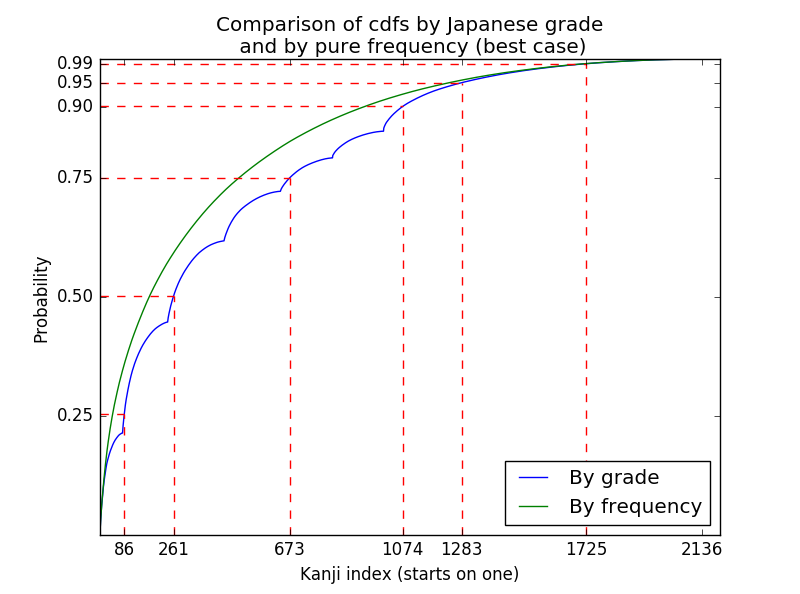
\includegraphics[width=\linewidth]{Cap2/CDFVersusGrade}
    \caption{Best case scenario.}
    \label{fig:cdfcomparisonbest}
    \end{subfigure}
    \begin{subfigure}{0.9\textwidth}
    \centering
    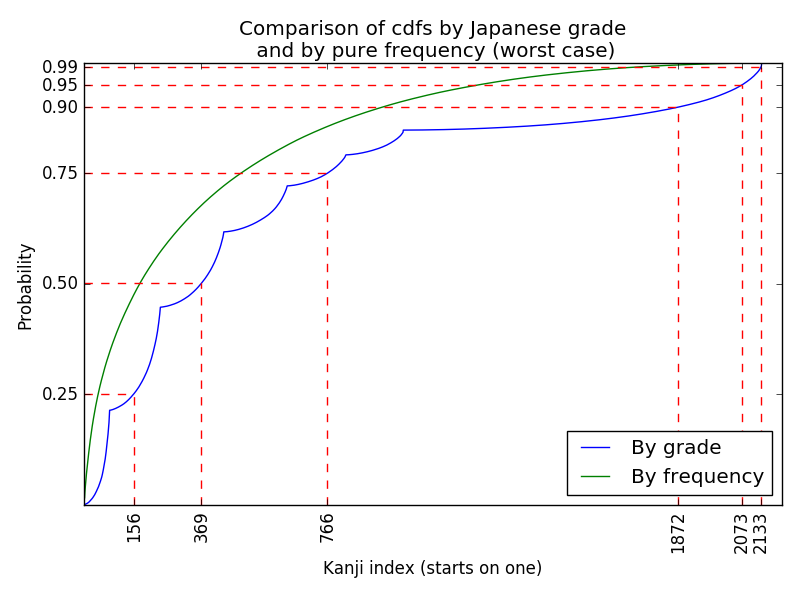
\includegraphics[width=\linewidth]{Cap2/CDFVersusGradeWorst}
    \caption{Worst case scenario.}
    \label{fig:cdfcomparisonworst}
    \end{subfigure}
    
    \caption{Comparison of the cumulative distribution functions bounded by grade and ordered solely through frequency.}
    \label{fig:cdfcomparison}
\end{figure}

In this case, the reference marks are used to depict the same reference probabilities as before, so that an effective comparison can be drawn between these two methods. The interpretation of these discrepancies are evaluated in the next Section.

\clearpage

\section{Kanji Probability Distribution Interpretation}\label{freqs:interpretation}

To better understand the information that can be drawn from these graphs, first we need to understand what does this cumulative probability distribution represents. An intuitive enunciation of the properties that follow from this analysis can be stated as follows:

\begin{center}
    "If I follow a certain strategy \textit{S} and have already studied \textit{N} Kanji, I'll have \textit{P} probability of having already studied a Kanji chosen arbitrarily in a random Japanese novel"
\end{center}

With this intuition, we can interpret the markings under the reference lines as the number of Kanji that should be studied if we want to know a certain percentage of characters that could be shown to us in a Japanese novel. A condensation of the information presented in Figures \ref{fig:cdfkanji} and \ref{fig:cdfcomparison} are put forward in Table \ref{tab:cdfcomparison}.

\begin{table}[ht]
\centering
\caption{Comparison of Kanjis to be studied to the same cumulative probabilities under different strategies}
\label{tab:cdfcomparison}
\begin{tabular}{|c|c|c|c|}
\hline
\multirow{2}{*}{\textbf{\begin{tabular}[c]{@{}c@{}}Probability of\\ having studied\end{tabular}}} & \multicolumn{3}{c|}{\textbf{Number of Kanji studied on Strategy}} \\ \cline{2-4} 
 & \textbf{Frequency} & \textbf{\begin{tabular}[c]{@{}c@{}}By Grades\\ (best case)\end{tabular}} & \textbf{\begin{tabular}[c]{@{}c@{}}By Grades\\ (worst case)\end{tabular}} \\ \hline
25\% & 44 & 86 & 156 \\ \hline
50\% & 175 & 261 & 369 \\ \hline
75\% & 493 & 673 & 766 \\ \hline
90\% & 939 & 1074 & 1872 \\ \hline
95\% & 1239 & 1283 & 2073 \\ \hline
99\% & 1720 & 1725 & 2133 \\ \hline
\end{tabular}
\end{table}

Firstly, we should appreciate the difference in proportions for the most efficient way of study by studying the first two columns of the table. For example, we note that by studying a total of 8.2\% (175) of the total number of Kanji we are already able to recognize half of all the Kanji occurrences in a Japanese novel. If we wish to be able to recognize 90\% of the Kanji, we only need to study a total of 44\% (939) of these. Furthermore, 99\% of occurrences are concentrated in 1,720 Kanji, leaving more than 400 Kanji sharing the last 1\% of occurrences. As we already commented in a previous Section, this distribution is not exactly Zipfian, but it does still follow a weak form of a Pareto rule, in a manner that an concentrated effort on the first few characters is much more justified than an indiscriminate study of Kanji.

By comparing columns two and three of Table \ref{tab:cdfcomparison}, we note that to reach 25\% of progress while following the Japanese grades but ordering them in the best case scenario, we will need to study roughly double the Kanji needed for the same probability in a study purely guided by frequency, which at this point are some measly 42 extra characters. This gap increases for 50\% and 75\% of probability, but closes down close to the end. This behaviour is attributable to the fact that that the last 1,133 are not divided in specific grades denominations, so that the gap between these two curves falls asymptotically after the inflection located at 84.8\% probability and 1,003 characters.

Now under the perspective of a unlucky student that follows the grade denominations but studies Kanji in the reverse order of their frequency, results are much more grim. To reach the mark of 25\% of probability of having studied an arbitrary character, this student needs to study 3.5 times more Kanji, or some extra 112 characters. This gap increases to almost 200 characters on 50\% probability, 273 for 75\%, 939 characters for 90\%, 834 characters for 95\% and 413 characters for 99\%. Note that at this point, the unlucky student would have studied 2,133 characters of the 2,136 total, leaving the last 1\% to be seen in the last three characters, a percentage that was dissipated among 416 characters in the best case.

A list with the ordered Kanji in decreasing frequency obtained from the data collected on this chapter is presented in the appendix, on Table \ref{tab:listfrequency}.